%%%%%%%%%%%%%%%%%%%%%%%%%%%%%%%%%%%%%%%%%%%%%%%%%%%%%%%%%%%%%%%%%%%%%%%%%%%%%%%%
%% 
\cleardoubleoddpage%  Make sure to start each chapter on a new odd page
\chapter{Theoretical Background}

\section{Respiratory Sounds}
\label{theory:sounds}
The respiratory system, which includes the airways and lungs, plays a crucial role in gas exchange, a vital function in the human body. Respiratory sounds, created by airflow during breathing, can reveal a lot about respiratory health~\cite{earis1992lung}. These sounds, observed through a process called 'auscultation'—listening to the chest with a stethoscope—are critical for detecting respiratory diseases. This method is cost-effective, non-invasive, and a standard part of physical examinations~\cite{bohadana2014fundamentals}.\\
We can categorize respiratory sounds into normal and anomalous based on their characteristics during auscultation. Normal sounds are typically heard during inhalation and at the start of exhalation, within a frequency range of 100 to 1000 Hz~\cite{bohadana2014fundamentals}. In contrast, abnormal sounds come in various forms. Here, we will discuss two common types: Wheezes and Crackles.\\\\
\textbf{Wheezes} are long and musical sounds that last over 100 milliseconds. They occur during inhalation and exhalation, often caused by narrowed or restricted airways. Their frequency usually falls between 100 to 1000 Hz, but higher harmonics are also possible~\cite{bohadana2014fundamentals}.\\\\
\textbf{Crackles}, conversely, are brief, non-musical sounds that signal sporadic airway openings, often due to secretions. We can further divide them into Fine and Coarse Crackles. Fine Crackles are short, with a frequency of around 650 Hz and a duration of about five milliseconds. Coarse Crackles last longer, over 15 milliseconds, and occur at lower frequencies, below 350 Hz~\cite{bohadana2014fundamentals}.\\\\
Understanding these distinctions in pulmonary sounds is vital for developing automated systems for their detection. Electronic stethoscopes can convert lung sounds into digital signals, enabling the use of advanced anomaly detection algorithms in computer-aided medical diagnosis.

\subsection{Digital Representation of Sound}
Sound signals, variations in air pressure known as sound waves, can be digitally represented in several ways. The following will give an overview of the used methods in this thesis.\\\\
\textbf{Waveforms} are the most straightforward representation, where the sound signal is a sequence of numbers $\mathbf{x}_n$ representing air pressure at time step $n\in \mathbb{N}$. The key parameter here is the sampling rate, which dictates how often the audio signal is sampled per second~\cite{backstrom2020introduction}.\\\\
\textbf{Spectrogram} representations, unlike waveforms, allow for a visual examination of the sound signal. This involves transforming the signal from a real-valued time-domain to a complex-valued frequency-domain representation using the Discrete Fourier Transform (DFT), mathematically defined as \[ X_k=\sum_{n=0}^{N-1}x_ne^{-i2\pi\frac{k\times n}{N}} \]. The result of this transformation provides a good overview of the frequencies that make up the sound signal. However, we are more interested in local events for non-stationary signals like respiratory sounds.\\
The Short Time Fourier Transform (STFT) helps obtain a representation that summarizes the sound signals' constituting frequencies while showing local changes in their distribution. It first divides the signal into short slices, also called windows. It then applies a windowing function to each slice, gradually reducing the signal amplitude towards the edges. This continuity between the windows is crucial for minimizing spectral leakage, a phenomenon where sudden changes in the signal between the windows get misinterpreted as sudden changes in the original signal. Finally, STFT involves applying a DFT on every window. We obtain a time-frequency representation typically visualized by converting $X_k$ to the log-spectrum $20log_{10}||X_k||$~\cite{backstrom2020introduction}.\\
Mel-Spectrograms refine this representation by aligning frequencies to the mel scale, approximating human hearing perception. This transformation is mathematically expressed as $m=2595log_{10}\left(1+\frac{f}{700}\right)$ as formulated by O'Shaughnessy (1987)~\cite{o1987speech}.\\\\
% Image for Spectrogram
\textbf{Mel-Frequency Cepstral Coefficients (MFCCs)} are used for dimensionality reduction in spectrograms to preserve essential information while reducing the number of coefficients. The process involves performing DFT on the waveform, computing the log amplitude spectrum, transforming the spectrum to the mel scale, and finally applying the Discrete Cosine Transform, a simplified version of the DFT resulting in a real-valued representation~\cite{backstrom2020introduction}. While not easily interpretable by humans, the resulting cepstrum is highly relevant for input into machine learning algorithms.

\section{Fundamentals of Anomaly Detection}
Anomaly detection is a process that identifies data points deviating from expected patterns, known as anomalies or outliers~\cite{chandola2009anomaly}. These deviations often signal critical changes in a system, requiring intervention. In healthcare, as discussed in \autoref{theory:sounds}, anomalies in respiratory sound patterns can indicate various conditions.\\
Anomaly detection algorithms characterize normal behavior, flagging deviations as anomalies. However, the rarity of anomalies and the uncertainty in their distribution poses significant challenges. Because anomalies are much more infrequent by nature, datasets typically are heavily unbalanced and contain a much larger number of normal samples than anomalies. Furthermore, the anomalous data points can exhibit various forms of non-normality, meaning there can be a substantial variation within the set of outliers~\cite{pang2021deep}. It is also essential to balance false positives and negatives based on the specific application domain.\\
Outlier detection can be categorized based on the data available:
\begin{enumerate}
  \item \textbf{Supervised Anomaly Detection}: This method uses a fully labeled dataset to differentiate between normal and abnormal data points. However, the lack of thorough datasets representing all the variance in anomalies limits these approaches.
  \item \textbf{Unsupervised Anomaly Detection}: More common in real-world scenarios, this approach uses only normal data points, requiring the system to learn their defining characteristics autonomously.
  \item \textbf{Weakly Supervised Anomaly Detection}: This approach, which we focus on in our research, uses primarily normal data points with a significantly smaller subset of anomalies. It is advantageous as it requires fewer anomalous data points than fully supervised methods while allowing for generalization abilities.
\end{enumerate}
Anomaly detection algorithms may provide a direct classification of data points as normal or anomalous or output an anomaly score indicating deviation from normality. This score helps identify anomalous samples by finding a threshold above which all samples can be considered anomalous. Traditional methods like K-nearest neighbor (KNN) and Support Vector Machines (SVMs) rely on distance metrics or decision boundaries to identify outliers. KNN works by identifying data points significantly distant from the closest set, while SVMs create a boundary between classes, effective in scenarios with clear separation~\cite{chandola2009anomaly}.\\
However, these traditional methods can be limited in handling complex, high-dimensional, and noisy data or when anomalies closely resemble normal data. Deep learning methods can extract features from raw data and have shown remarkable effectiveness in learning complex patterns, such as those in audio signals. We will explore two distinct deep-learning architecture families used in this research, highlighting their suitability for anomaly detection in respiratory sounds.

\section{Reconstruction-Based Methods}
Reconstruction-based methods in anomaly detection use reconstruction errors as anomaly scores to identify anomalies. These methods involve two primary steps: dimensionality reduction and data reconstruction. Initially, the data is transformed into a latent, more compact representation in a latent space. This space aims to retain essential data features while discarding noise and irrelevant details. The subsequent step involves reconstructing the original data from this compact representation. The core challenge lies in achieving a balance where the reduced representation is compact yet retains sufficient information for accurate reconstruction without overfitting.\\
These models are trained unsupervised, using only normal data points. This approach ensures that the model learns typical patterns of such. The reconstruction error is calculated during training, reflecting the accuracy with which the model can recreate the input data. The underlying assumption is that a model trained on normal data will yield minimal error in reconstructing similar data. However, when encountering anomalous data that deviates from learned patterns during evaluation or inference, the model faces difficulties in reconstruction, resulting in a higher reconstruction error. This error then serves as an anomaly score, with higher errors indicating a greater likelihood of anomaly and vice versa.

\subsection{Essentials of Autoencoders}
Autoencoders are a prevalent neural network architecture in reconstruction-based methods, known for their ability to learn compact data representations unsupervised. An autoencoder comprises two main components: the Encoder and the Decoder.\\
\begin{itemize}
  \item \textbf{Encoder} ($A:\mathbb{R}^n \rightarrow{} \mathbb{R}^l$): This component maps high-dimensional input data (dimensionality $n$) into a lower-dimensional latent space (dimensionality $l<n$). This process compresses the data into an efficient, compact form.
  \item \textbf{Decoder} ($B:\mathbb{R}^l \rightarrow{} \mathbb{R}^n$): The Decoder performs the inverse function, reconstructing data from the latent space back to its original dimensionality. Its goal is to replicate the original input as closely as possible.
\end{itemize}
The optimization challenge in autoencoders can be formulated as follows:
\[ \text{arg min}_{A,B}E[\Delta (\mathbf{x}, B \circ A(\mathbf{x}))], \]
where $E$ represents the expected value of the reconstruction loss $\Delta$ for input $\mathbf{x}$~\cite{bank2023autoencoders}.

% Maybe add an illustration

\section{Density Estimation Methods}
Density estimation methods in anomaly detection revolve around the concept of probability distributions. Probability distributions are mathematical functions that describe the probability associated with each possible value of a random variable. Suppose the random variable can take any value within a specific range. In that case, the probability distribution is continuous and can be described by a Probability Density Function (PDF), providing a probability of a random variable falling within a specific range.\\
For a continuous real-valued random variable $X$, the PDF is defined as
\[ P(a\leq X\leq b)=\int_a^bf(x)dx \]
for all $ a, b \in \mathbb{R}$~\cite{grinstead2006probabilities}. Here, $f(x)$ represents the probability density function of $X$. It is important to note that the PDF does not give probabilities directly. Instead, the area under the PDF curve between these points gives the probability of $X$ falling within the interval from $a$ to $b$.\\
Density estimation involves estimating the PDF from observed data by estimating a joint distribution $ p(\mathbf{x}) $ from a set of examples $ \{ \mathbf{x}^{(t)}\}^T_{t=1}$~\cite{germain2015made}. The estimation can be parametric, where the data is assumed to follow a known distribution like Gaussian with the mean and standard deviation as parameters, or nonparametric, which does not presume a specific distribution and directly estimates the PDF from the data. Nonparametric methods can handle more complex distributions but usually require more data to produce an accurate estimate.\\
In anomaly detection, estimating the PDF of a dataset helps identify regions of low probability. Data points in these regions are potential anomalies, making density estimation a powerful tool for detecting outliers.


% Maybe include a graphic showing the distribution
\subsection{Introduction to Masked Autoencoders}
\label{theory:made}
Masked Autoencoders for Distribution Estimation (MADE) extend the concept of autoencoders so that they can understand the data distribution. Unlike traditional autoencoders, MADE enforces the autoregressive property and considers the input data order so that each output part is influenced only by preceding input parts.\\
The autoregressive property is accomplished by masking the weights in each autoencoder layer, controlling the information flow. Each neuron is labeled with a number from $1$ to $D-1$ (where $D$ is the input dimensionality) and the following rule is applied to determine allowed connections: a neuron in layer $l$ (called $k'$) can only be connected to a neuron in the previous layer $l-1$ (called $k$) if its label is greater than or equal to the label of $k$. Mathematically, Germain et al. (2015) states this concept as
\[ M^{\mathbf{W}^l}_{k',k}=\begin{cases}
    1, & \text{if } m^l(k')\geq m^{l-1}(k) \\
    0, & \text{otherwise.}
  \end{cases} .\]
Here, $M^{\mathbf{W}^l}_{k',k}$ is the weight matrix mask that determines whether a connection is allowed or not. For the output layer, the rule needs the slight modification of making the condition strict ($m^l(k')> m^{l-1}(k)$) to maintain the autoregressive property.\\
MADE's architecture allows for calculating the probability of observing the input $\mathbf{x}$ as
\[ p(\mathbf{x}) = \sum_{d=1}^{D} p(x_d | \mathbf{x}_{<d}) .\]
This probabilistic model is beneficial in anomaly detection as it can identify data points with low probability, indicating potential anomalies.

% Include Benefits
% Include graphic that shows the probabilities being output can be used to get p(x)

\section{Evaluation Metrics for Model Comparison}
Evaluating and comparing the performance of different anomaly detection models requires carefully chosen metrics relevant to real-world applications and offers clear, intuitive interpretations of the models' effectiveness. Before introducing the five core metrics considered in this thesis, we need to understand the concept of a confusion matrix.
In anomaly detection, we can categorize a model's prediction outcome into four types: true negatives (correct normal prediction), false negatives (anomalies incorrectly labeled as normal), true positives (correct anomaly prediction), and false positives (normal data points mistakenly identified as anomalies). A confusion matrix summarizes these four outcomes.\\
Having introduced the needed terminology, we focus on defining the evaluation metrics.
% Add graphic of a confusion matrix

\subsubsection{Sensitivity (True Positive Rate - TPR)}
\[ TPR=\frac{TruePositives}{TruePositives+FalseNegatives}. \]
Sensitivity measures the proportion of actual anomalies correctly identified. It ranges from 0 (no anomaly detected) to 1 (perfect anomaly detection), with a higher value preferable, especially in critical applications like healthcare, where leaving an anomaly undetected can have serious implications.

\subsubsection{False Positive Rate (FPR)}
\[ FPR=\frac{FalsePositives}{TrueNegatives+FalsePositives}. \]
FPR assesses the proportion at which normal data points are incorrectly classified as anomalies. It ranges from 0 (no false alarms) to 1 (all normal data classified as anomalies). A lower FPR is desired, as it indicates fewer false alarms.

\subsubsection{Specificity (True Negative Rate - TNR)}
\[ TNR=\frac{TrueNegatives}{TrueNegatives+FalsePositives} .\]
Specificity quantifies how well the model identifies normal data points. It also ranges from 0 (poor recognition of normal conditions) to 1 (excellent recognition of normal conditions). Higher specificity is essential to minimize false alarms in sensitive domains like medical settings.

\subsubsection{Area Under the Curve (AUC)}
The Area Under the Curve (AUC) is a metric calculated using the Receiver Operating Characteristic (ROC) curve, which portrays the True Positive Rate (TPR) against the False Positive Rate (FPR) within a unit square, with TPR on the Y-axis and FPR on the X-axis. This visualization emphasizes the trade-off between a model's capability to correctly identify anomalies (TPR) and its tendency to misclassify normal data as anomalous (FPR).\\

\begin{figure}[h!]
  \centering
  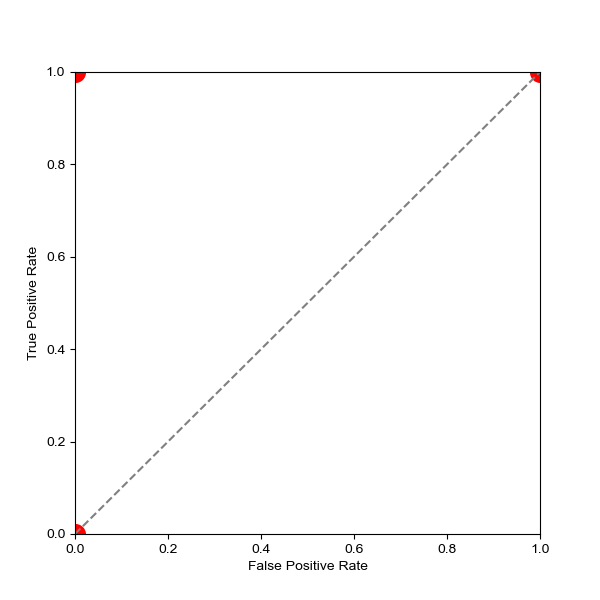
\includegraphics[width=0.5\linewidth]{images/rocauc}
  \caption{
  ROC curve, highlighting special points and diagonal
}
\end{figure}

In this graph, a point at (0,0) signifies a model that categorizes all data as normal, while (1,1) indicates a model labeling everything anomalous. The theoretical perfect model achieves flawless classification, represented by (0,1). The ROC curve emerges by systematically adjusting the model's classification threshold and plotting corresponding TPR and FPR values, forming a curve that illustrates performance across various thresholds~\cite{fawcett2006introduction}.\\
A random model aligns with the diagonal line from (0,0) to (1,1) in binary classification tasks like anomaly detection. Performance surpasses randomness when the ROC curve lies above this diagonal and diminishes when below. The AUC is a quantitative measure of this performance, quantifying the area enclosed by the ROC curve and the x-axis. It ranges from 0.5 (no discrimination ability) to 1 (perfect classification). Notably, models with an AUC below 0.5 can be adjusted to achieve better-than-random classification.\\
A high AUC is crucial in medical diagnostics to detect pathologies while avoiding false alarms and overtreatment of healthy patients.

\subsubsection{Balanced Accuracy (BALACC)}
Balanced Accuracy (BALACC) assigns equal importance to correctly identifying anomalies and normal data points. It is calculated as the average of Sensitivity (True Positive Rate) and Specificity (True Negative Rate):
\[ BALACC=0.5 \times (Sensitivity + Specificity) \]
This metric is especially useful in scenarios where the dataset is unbalanced, a common occurrence in anomaly detection where anomalies are much rarer than normal samples. In such cases, traditional accuracy metrics can be misleading. For example, consider a dataset where 95\% of the data points are normal and only 5\% are anomalies. A model that naively classifies every data point as normal would achieve a 95\% accuracy rate, which is misleadingly high. Balanced Accuracy corrects this distortion by considering both the ability to detect anomalies (sensitivity) and recognize normal instances (specificity), providing a more truthful measure of a model's performance. In our example, it would only result in a 50\% Balanced Accuracy.\\
Balanced Accuracy has a goal similar to the AUC's: correctly identifying diseased and healthy individuals.



%% 
%%%%%%%%%%%%%%%%%%%%%%%%%%%%%%%%%%%%%%%%%%%%%%%%%%%%%%%%%%%%%%%%%%%%%%%%%%%%%%%%